\subsection{Two-flow dumbbell, repetition 1}
\begin{figure}[H]\centering
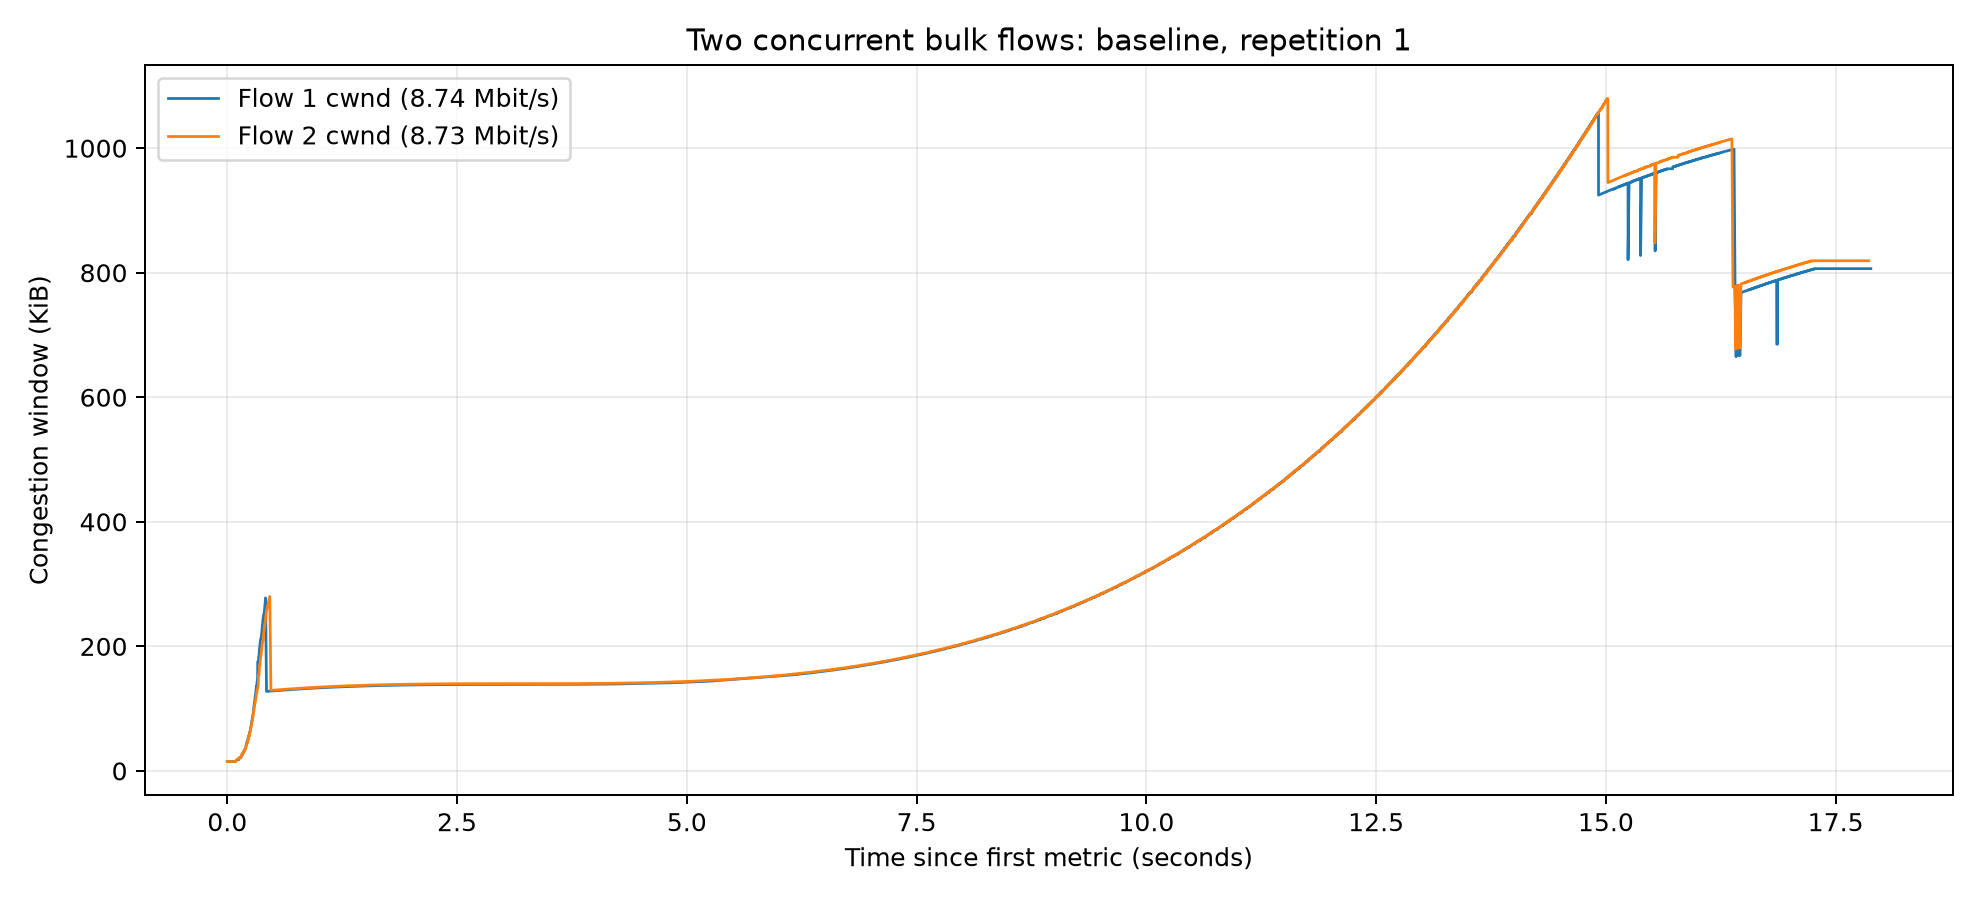
\includegraphics[width=0.92\textwidth]{plots/dumbbell/baseline-1.png}
\caption{Baseline: both client/server pairs transfer 20 MiB concurrently over the shared bottleneck.}\end{figure}
\begin{figure}[H]\centering
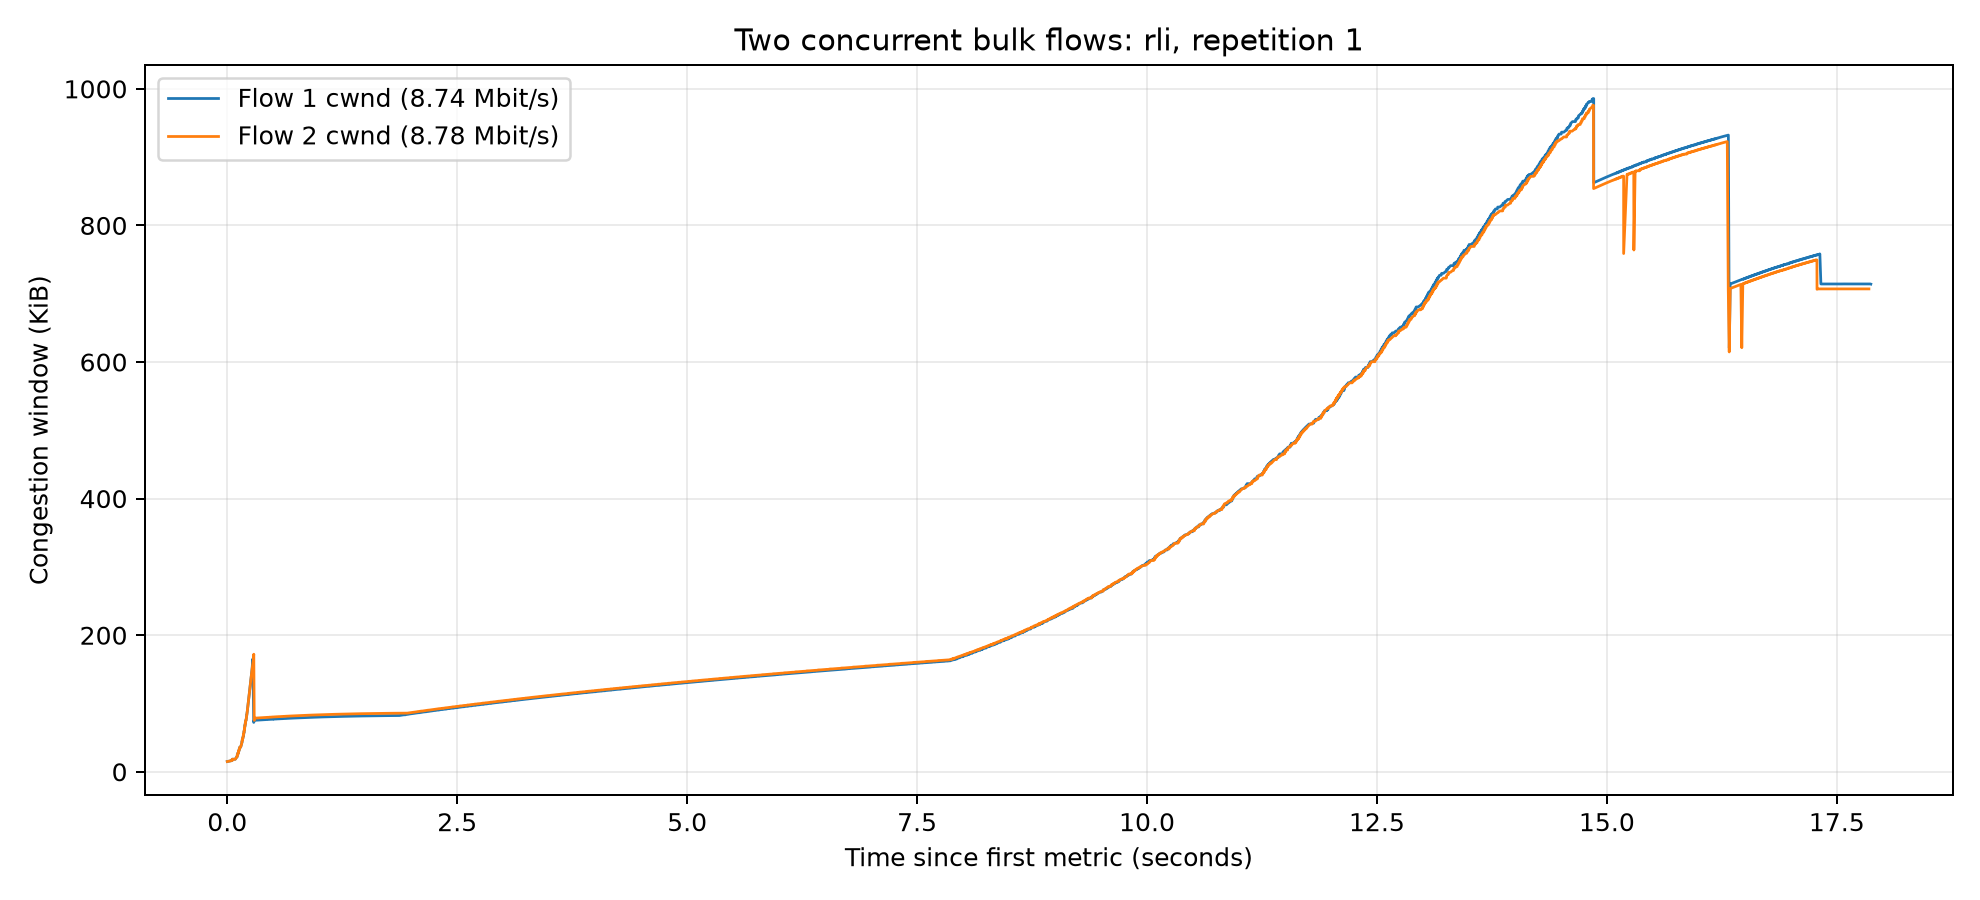
\includegraphics[width=0.92\textwidth]{plots/dumbbell/rli-1.png}
\caption{Rli: both client/server pairs transfer 20 MiB concurrently over the shared bottleneck.}\end{figure}
The two lines show the congestion windows of competing flows. Window height and temporary differences in allocation should be interpreted alongside the transfer rates and Jain index.
\clearpage\subsection{Two-flow dumbbell, repetition 2}
\begin{figure}[H]\centering
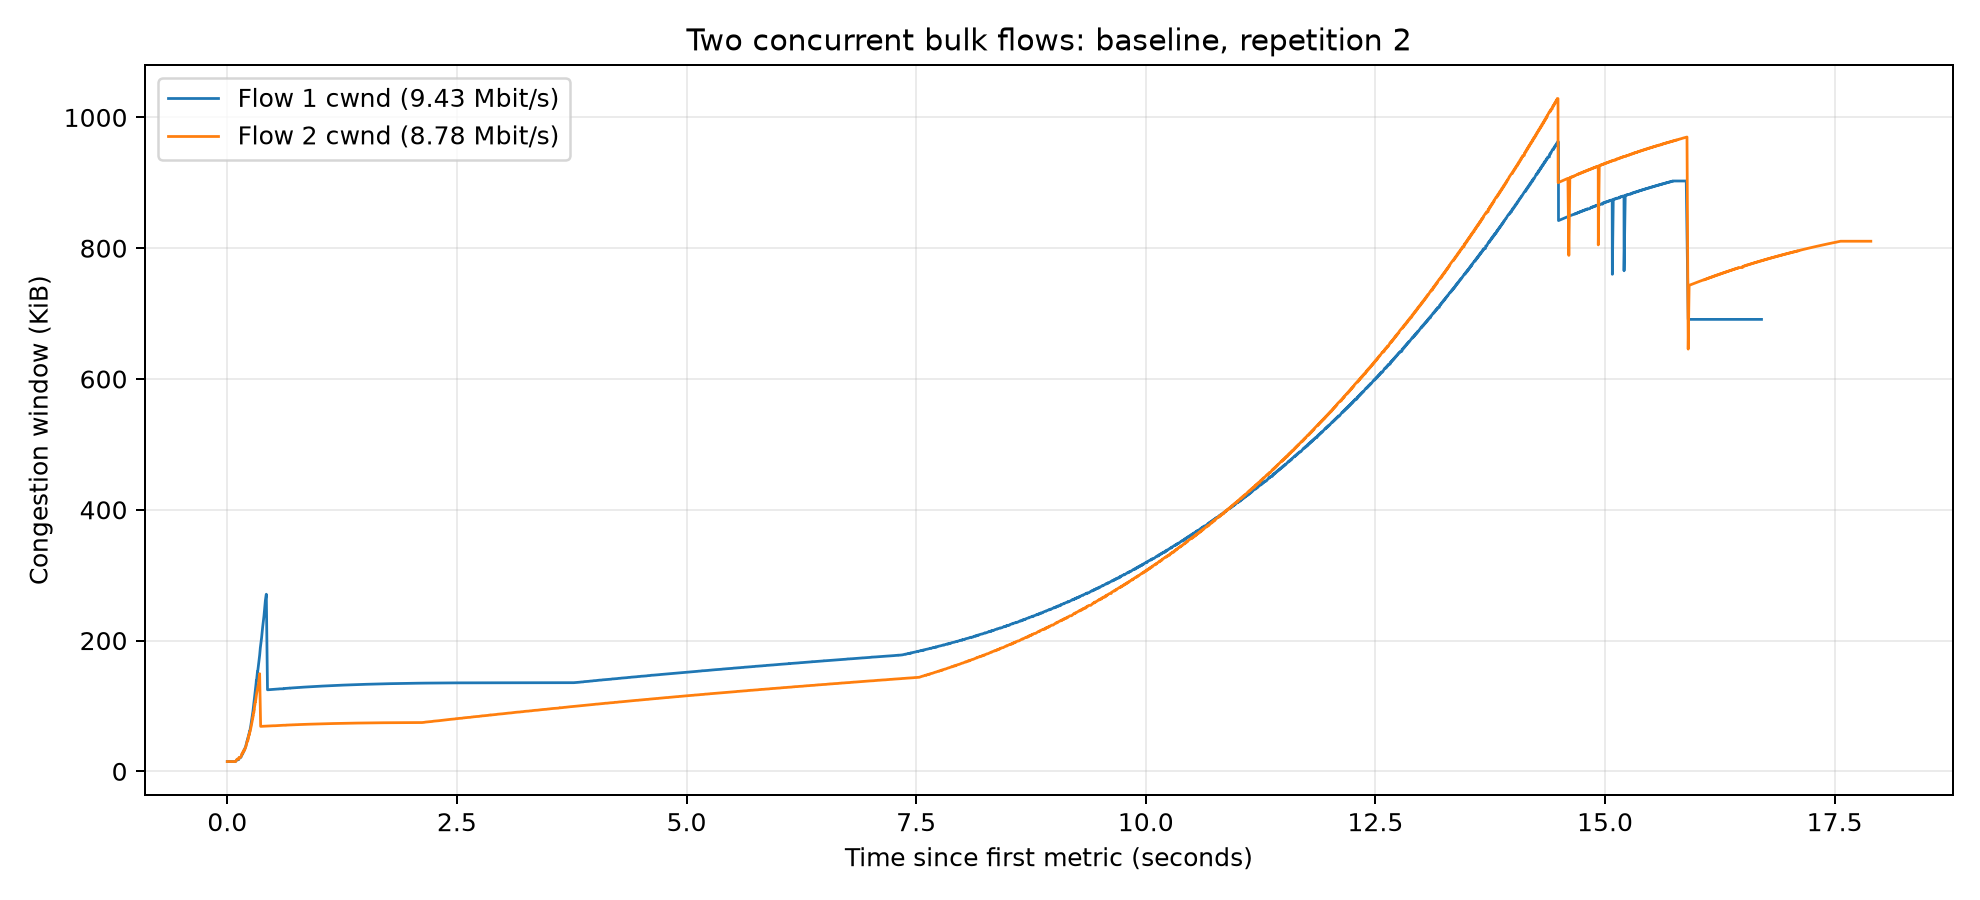
\includegraphics[width=0.92\textwidth]{plots/dumbbell/baseline-2.png}
\caption{Baseline: both client/server pairs transfer 20 MiB concurrently over the shared bottleneck.}\end{figure}
\begin{figure}[H]\centering
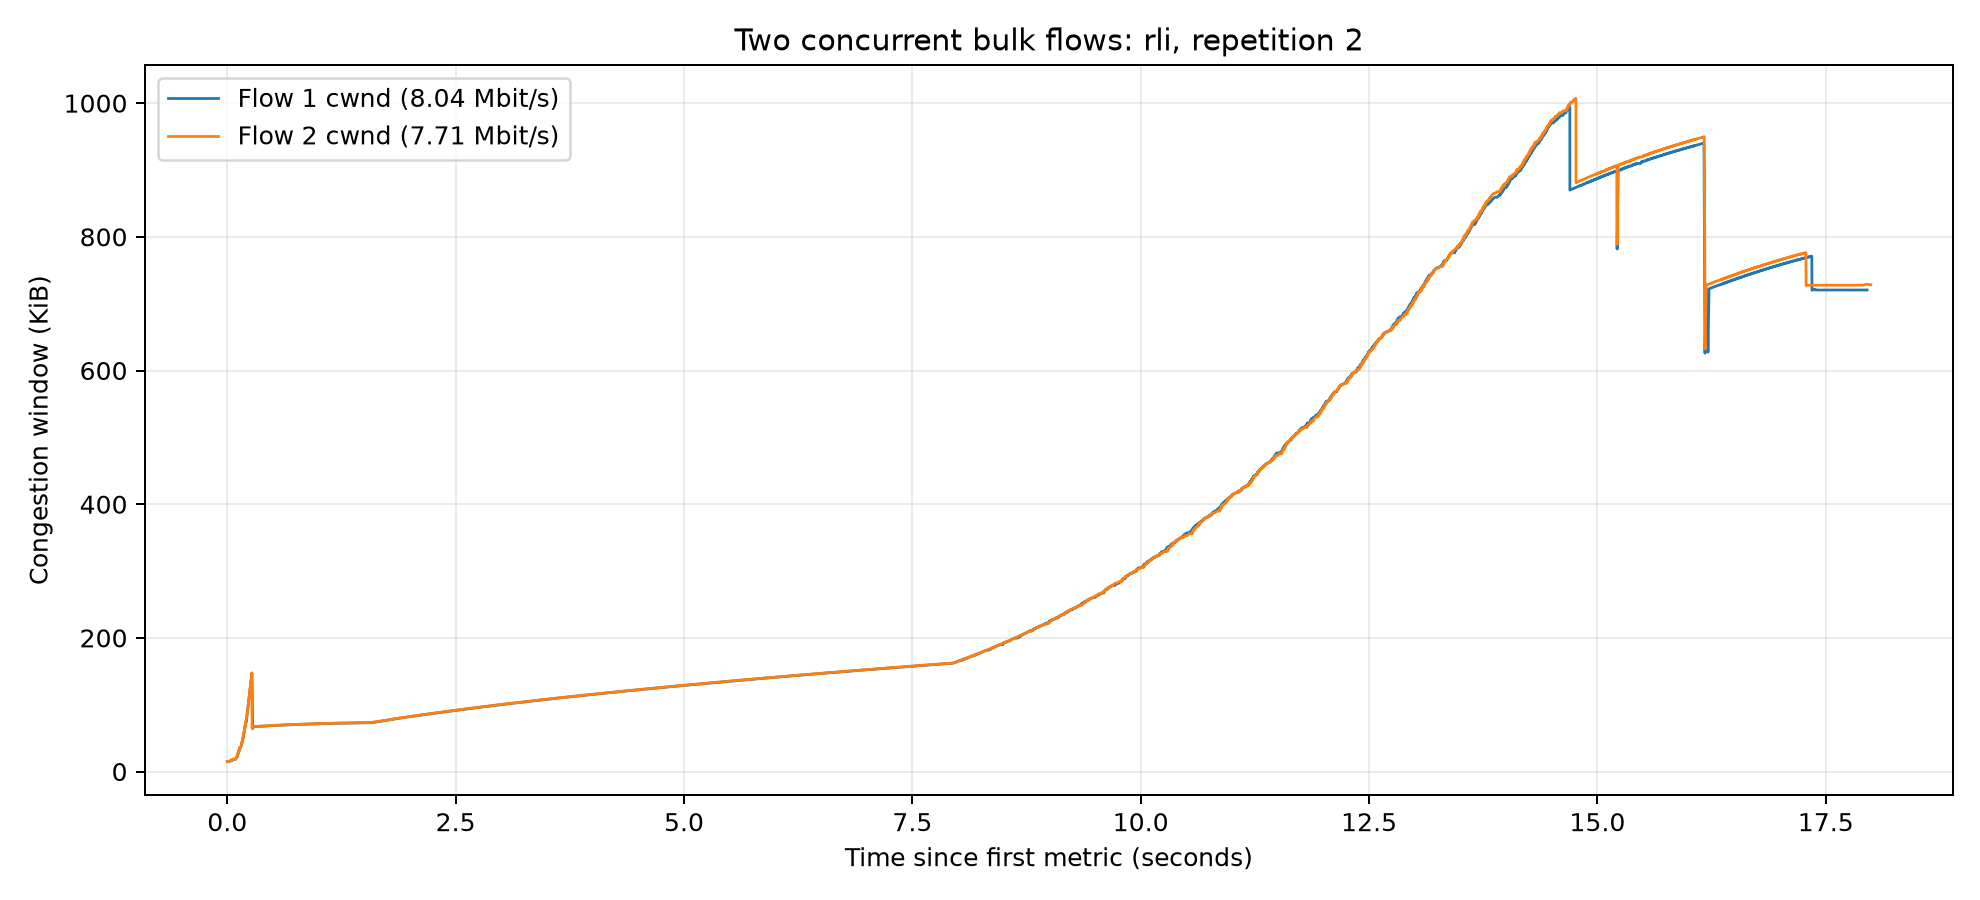
\includegraphics[width=0.92\textwidth]{plots/dumbbell/rli-2.png}
\caption{Rli: both client/server pairs transfer 20 MiB concurrently over the shared bottleneck.}\end{figure}
The two lines show the congestion windows of competing flows. Window height and temporary differences in allocation should be interpreted alongside the transfer rates and Jain index.
\clearpage\subsection{Two-flow dumbbell, repetition 3}
\begin{figure}[H]\centering
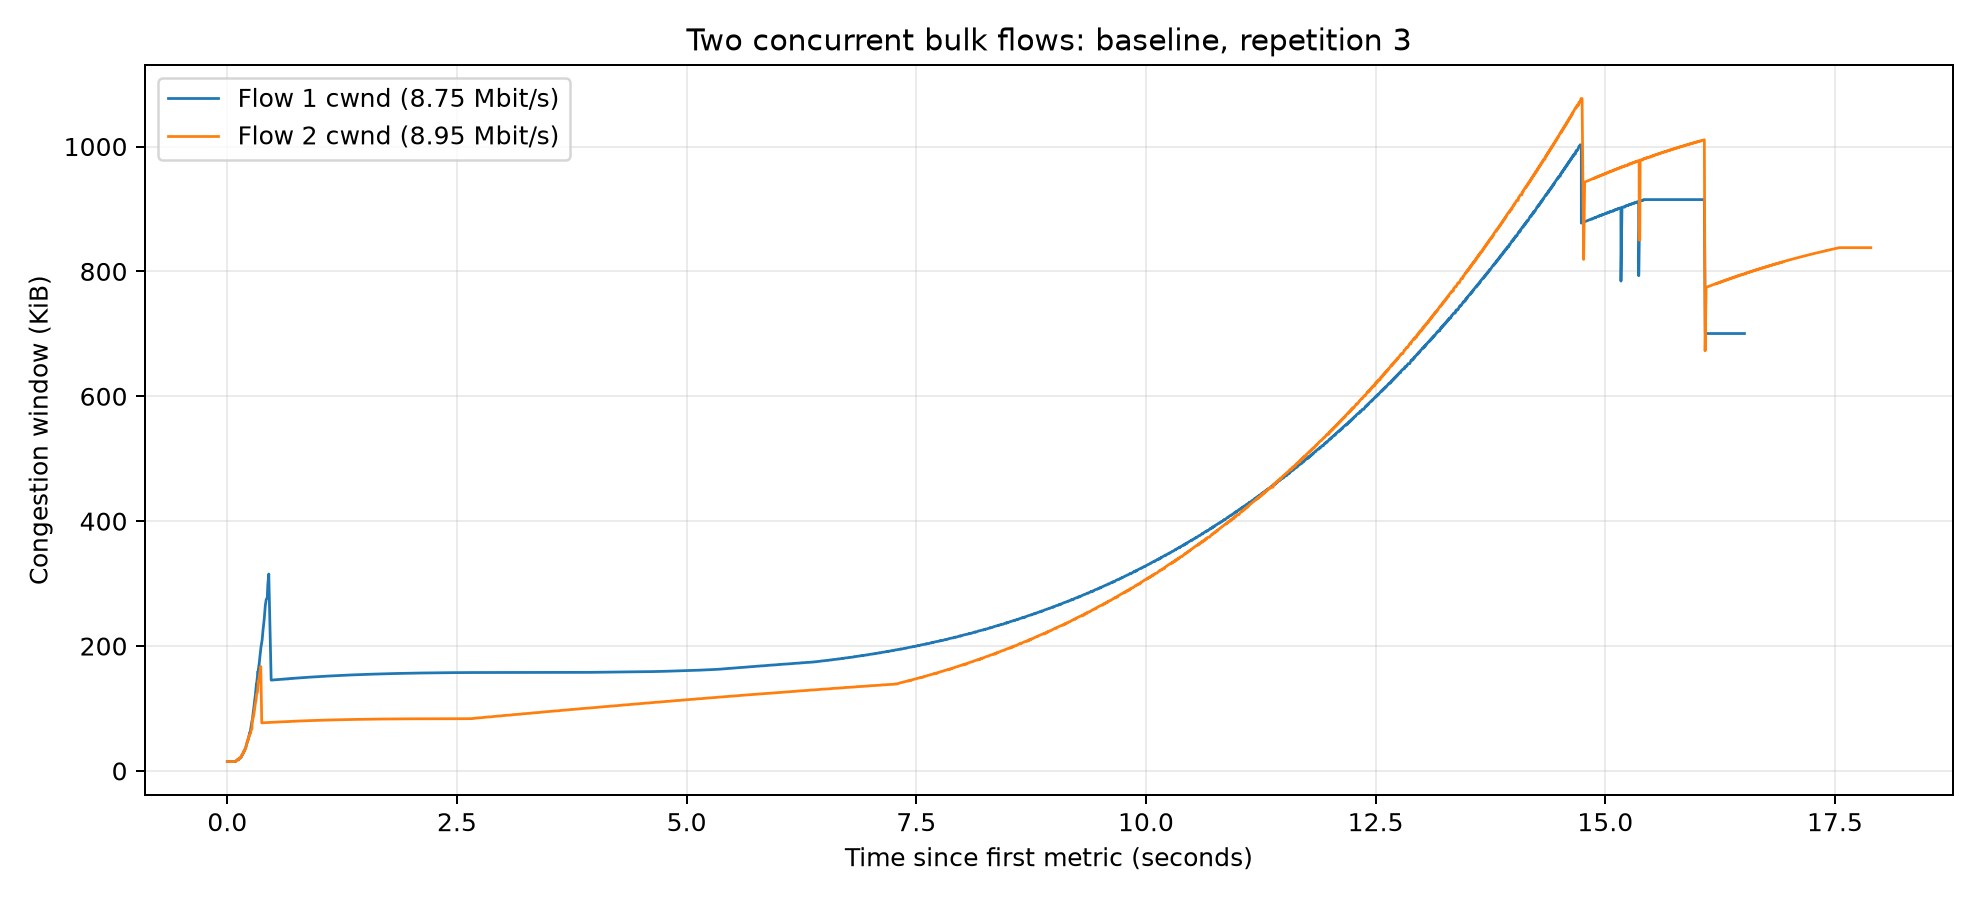
\includegraphics[width=0.92\textwidth]{plots/dumbbell/baseline-3.png}
\caption{Baseline: both client/server pairs transfer 20 MiB concurrently over the shared bottleneck.}\end{figure}
\begin{figure}[H]\centering
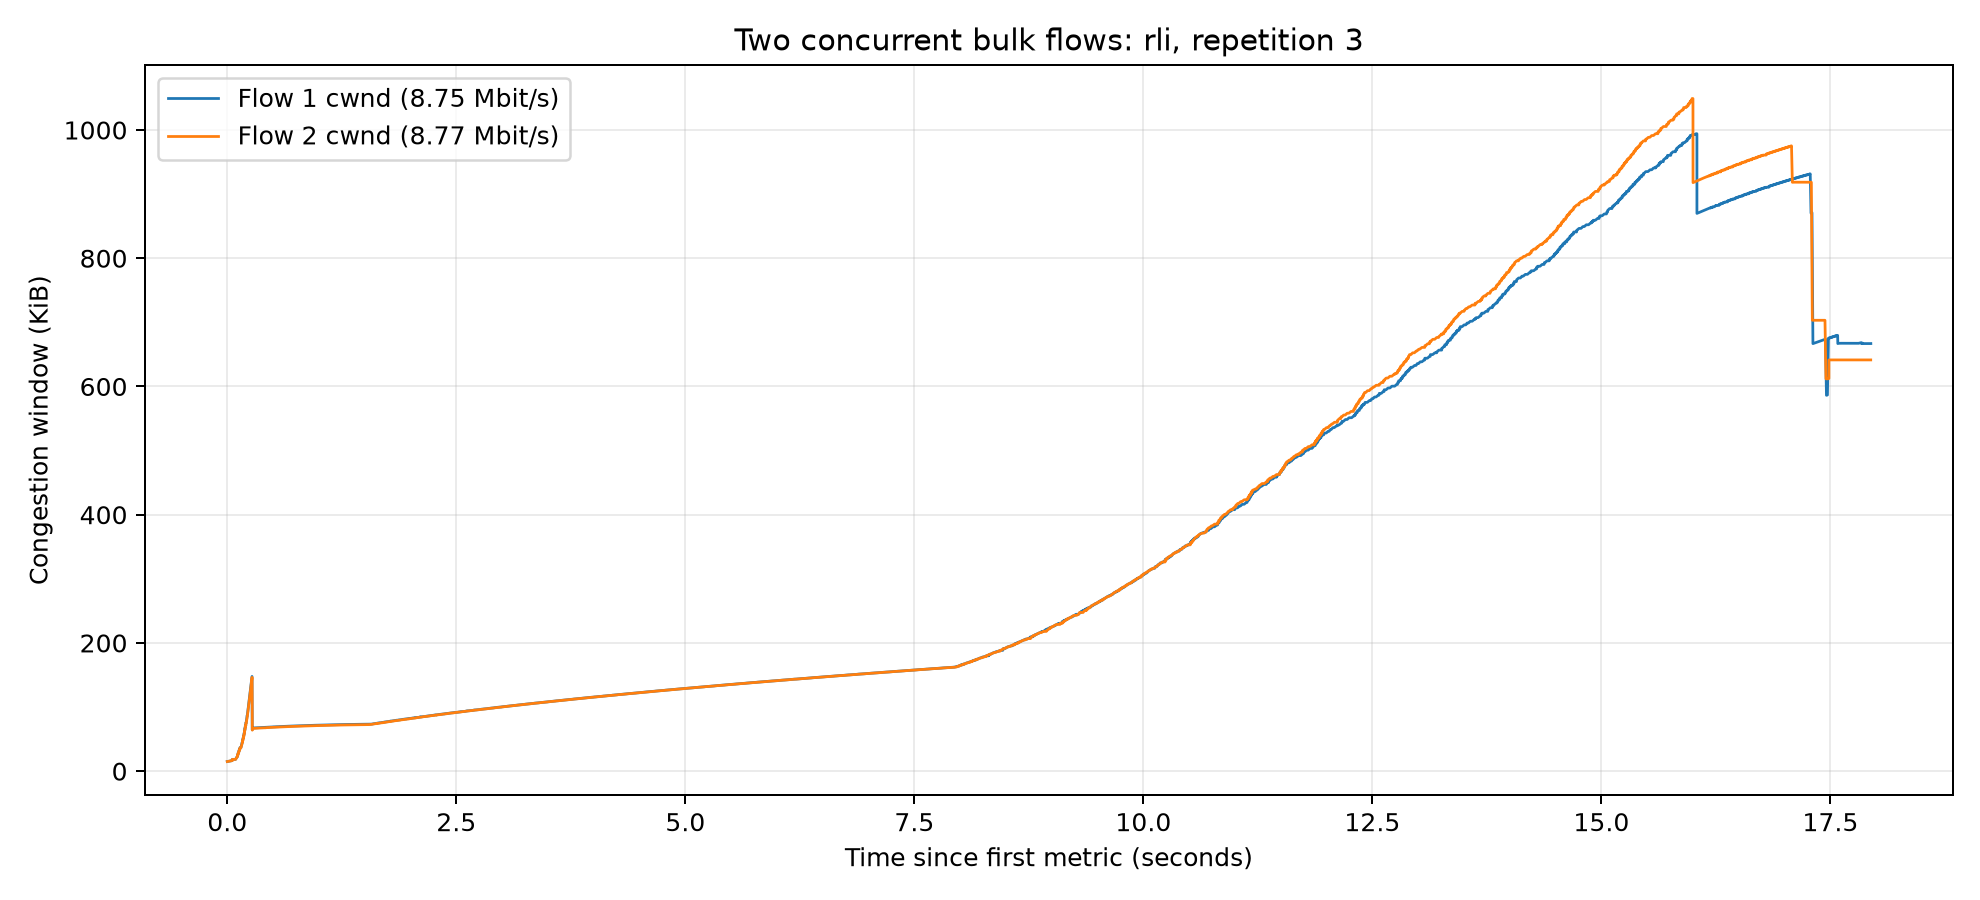
\includegraphics[width=0.92\textwidth]{plots/dumbbell/rli-3.png}
\caption{Rli: both client/server pairs transfer 20 MiB concurrently over the shared bottleneck.}\end{figure}
The two lines show the congestion windows of competing flows. Window height and temporary differences in allocation should be interpreted alongside the transfer rates and Jain index.
